
\chapter{Introdução}

\label{CapIntro}

% Resumo opcional. Comentar se não usar.
\resumodocapitulo{O desenvolvimento tecnológico culminou na demanda por melhorias de serviços que, outrora, não eram capazes de integrar os fatores aliados à facilidade e ao bem-estar dos usuários. O bem-estar, dentro de edifícios, está associado diretamente ao conforto ambiental. Esse conceito é estudado nos ramos de arquitetura e construção civil e visa a garantia das condições que possibilitam a qualidade física e psicológica dos indivíduos dentro dos mais diversos ambientes e instalações.}

\section{Contextualização}

O momento em que se elabora este projeto é uma época de grandes mudanças em quesitos de tecnologia. O entendimento do impacto ao meio ambiente, gerado pelo consumo energético em residências, estabelecimentos comerciais e fabris começa a ser compreendido por boa parte das pessoas, e principalmente o conhecimento da escalabilidade do impacto individual das pessoas de uma população.

Nas últimas décadas, a racionalização do consumo energético vem sendo alvo de diversos encontros técnicos da área de sustentabilidade, e de diversos acordos globais para a redução das emissões de carbono, geradas principalmente, devido à ação humana, especialmente na produção de energia.

Ao mesmo tempo em que o consumo é questionado, as exigências quanto à qualidade de vida, segurança no trabalho, ergonomia e conforto passaram a ser aspectos chave na vida e no dia-a-dia das pessoas. Seja no trabalho, ou no ambiente domiciliar, o conforto térmico é decisivo para o bem-estar das pessoas, assim como para a produtividade no ambiente de trabalho.

É um desafio alcançar a completude do conceito de conforto ambiental nas edificações. Nesse sentido, a automação é capaz de otimizar situações de uso de instrumentos cotidianos para vantagens como: a facilitação de trabalhos, muitas vezes manuais, para a economia de energia, para o estabelecimento de relações automáticas entre duas variáveis, a exemplo da entrada de pessoas em uma sala e o acionamento do ar condicionado, dentre outras vantagens.

\subsection{Conforto ambiental}

Conforto Ambiental é um conjunto de condições que possibilitam o bem-estar físico e psicológico dos indivíduos em diferentes locais, sendo que, o enfoque deste trabalho é principalmente em relação ao interior de instalações.

Esse conforto pode ser subdividido em categorias como: visual (abrangendo iluminação e estética visual), ergonômico (que tem muito destaque na parte de segurança do trabalho e com exemplos claros de esforços repetitivos, etc.), acústico (onde há limites em decibéis muito bem definidos) e térmico, que se configura como objeto desse trabalho. As normas vigentes que regem a construção e habitação de ambientes quanto ao aspecto de conforto ambiental e térmico são a ANSI/ASHRAE \textit{Standard} 55-2017 \cite{ASHRAE} e as NBRs 15.575 \cite{NBR15575} e 15.220 \cite{NBR15220}.

Nesse sentido, tecnologias de comunicação sem fio, como o RFID - que será melhor explicado no decorrer deste projeto – podem ser utilizadas para o melhoramento interno (\textit{indoor}) de edifícios, proporcionando melhores condições para que seja possível atingir o conforto ambiental. A figura \ref{fig:image} demonstra a aplicação de tecnologias de controle e monitoramento para a aquisição de conforto interno.

\begin{figure}[H]
    \centering
    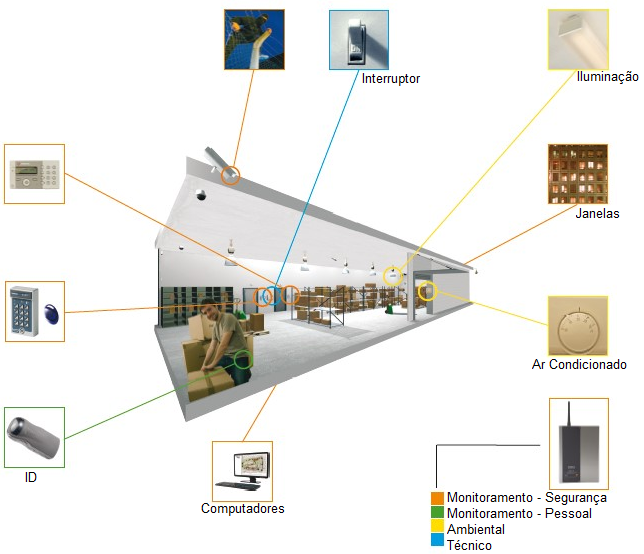
\includegraphics[width=0.6\linewidth]{figs/Introducao/imagem.png}
    \caption{Tecnologias de controle e monitoramento \textit{indoor} a fim de se atingir conforto ambiental. (Adaptado de 3DSecurity Systems \cite{imagem})}
    \label{fig:image}
\end{figure}


\subsection{Tecnologias de comunicação sem fio}

O uso de RFID, Bluetooth, Zigbee pode auxiliar na automação e possibilitar a instalação de sistemas de condicionamento baseados na movimentação (entrada e saída) de pessoas. Segundo Ahmed \textit{et al.} \cite{AhmedIntegrationStreamMapping}, sistemas de comunicação sem fio (\textit{wireless}) podem reduzir significativamente a frequência de erros humanos, otimizar a gestão e aumentar a acurácia da informação principalmente em relação à indoor network (rede interna). Chen \textit{et al.} \cite{chenUsingRFID}, retrata ainda, quão importante é a utilização de ferramentas como o RFID para a rastreabilidade e compra segura de alimentos. O uso de RFID pode ser empregado até no controle do fluxo de saída de roupas de uma loja.

Esses sistemas que funcionam à distância, sem fio, como o RFID, que é o sistema de identificação por radiofreqüência (RFID), que será melhor explicado no capítulo \ref{chap:Fundamentacao}, permitem recuperar informações armazenadas de um objeto preso ou incorporado a bens, produtos ou seres vivos \cite{gutierrez2005complexo}. Dessa forma, o emprego de tecnologias sem fio pode proporcionar a melhor administração de indivíduos em situações rotineiras e também em situações de emergência. 

\section{Trabalhos anteriores}

A elaboração deste projeto dá continuidade à uma sequência de trabalhos executados no Laboratório de Automação e Robótica da Universidade de Brasília (LARA - UnB). Em especial destacam-se o trabalho de Oliveira, Filipe e Rocha, Frederico \cite{TG2013OliveiraERocha} e o trabalho de Alves, Raissa e Chupel, Renata \cite{TG2015RaissaERenata}, este último a partir do qual dá-se continuidade.
Este trabalho estima obter uma nova abordagem aos equipamentos de RFID disponíveis no laboratório, para obter a identificação da quantidade de pessoas em um ambiente, através de um novo algoritmo, e uma nova disposição física dos equipamentos no laboratório.

\section{Proposta}

A proposta deste trabalho consiste em utilizar a tecnologia RFID passivo para estimar a quantidade de pessoas que ocupam um determinado ambiente. O cenário vislumbrado é de um edifício de escritórios, sala de aula, anfiteatro ou auditório, oficina ou fábrica, ou qualquer ambiente cuja definição exata da quantidade de pessoas que ocupam tal ambiente seja relevante.

A motivação principal para a elaboração do trabalho foi a estimação do impacto na carga térmica causado pelas pessoas que transitam e ocupam um ambiente fechado. O princípio almejado é realizar o controle de equipamentos de ventilação, aquecimento e ar-condicionado (HVAC - em inglês \textit{Heating, Ventilation and Air Conditioning}) de forma antecipada à variação das condições climáticas internas, em especial a temperatura e a umidade. Este propósito é considerado importante para sistemas de ar-condicionado simples e complexos, seja para manutenção do conforto térmico em um ambiente de trabalho, seja para minimizar a variação de temperatura em um ambiente onde as condições do ar são críticas, como uma sala de cirurgia ou laboratório, sala servidores ou \textit{datacenter}.

Este propósito pode ser extrapolado para aplicações de controle de acesso e segurança, como por exemplo, a definição de alarmes de intrusão de áreas restritas, alarmes de quantidade máxima de ocupantes por sala, ou rastreamento da trajetória de visitantes em um ambiente. Utiliza-se como exemplo um laboratório onde, para preservar as condições de limpeza, segurança e temperatura, limita-se o número de pessoas que pode transitar dentro deste ambiente por vez.

O principal objetivo deste trabalho é criar um espaço inteligente, que utiliza dados de tecnologias sem fio para aprimorar a qualidade de vida e de trabalho das pessoas, ao mesmo tempo em que proporciona economia de energia e segurança.

O objetivo específico do trabalho é desenvolver uma aplicação RAIN RFID para monitorar o trânsito de pessoas em um ambiente fechado e contabilizar a quantidade de pessoas presentes em cada subdivisão deste ambiente, em tempo real.

Esse trabalho apresenta, na fundamentação teórica (capítulo \ref{chap:Fundamentacao}), o embasamento dos conceitos: tecnologias comumente utilizadas, RFID e seus componentes, redes de Petri, efeito Doppler e localização \textit{indoor}.

À seguir, no capítulo \ref{chap:Metodos} de Metodologias, são apresentados os materiais utilizados e as abordagens para se atingir o objetivo do trabalho, que é o monitoramento de pessoas em ambientes fechados. A seção de abordagem utilizada (seção \ref{abordagem}) foi subdividida em: instalação física das leitoras e antenas, local de testes, elaboração do software, configuração das leitoras, transições e curvas de valores e os conceitos por trás dos seis métodos de monitoramento utilizados:

\begin{itemize}
    \item Comparação do último valor de RSSI capturado
    \item Comparação dos tempos dos últimos picos das curvas de RSSI
    \item Comparação das médias das curvas de potência RSSI
    \item Comparação das medianas das curvas de potência RSSI
    \item Utilização do efeito Doppler como critério de travessia de um ambiente para outro
    \item Combinação dos métodos de tempos de picos de valores RSSI e transição por efeito Doppler
\end{itemize}